\begin{figure}
  \centering
  \hspace*{-0.15\textwidth}%
  \begin{subfigure}[t]{0.125\textwidth}
    \tikzstyle{legend-point}=[circle, inner sep=1.25pt]
    \definecolor{GraphBlue}{HTML}{6c8abd}
    \definecolor{GraphGreen}{HTML}{73b584}
    \definecolor{GraphRed}{HTML}{d07175}
    \definecolor{GraphPurple}{HTML}{8172b2}
    \definecolor{GraphYellow}{HTML}{ccb974}
    
    \definecolor{legend1}{HTML}{eed0cd}
    \definecolor{legend2}{HTML}{deb1d4}
    \definecolor{legend3}{HTML}{aca3d8}
    \definecolor{legend4}{HTML}{72a2b5}
    \definecolor{legend5}{HTML}{549874}
    \definecolor{legend6}{HTML}{5d773b}
    \definecolor{legend7}{HTML}{6c4c2e}
    \definecolor{legend8}{HTML}{5c2b3d}
    \definecolor{legend9}{HTML}{311c3b}

    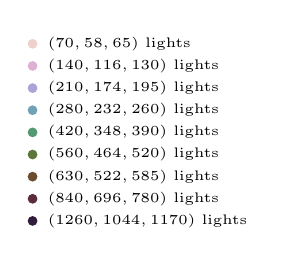
\begin{tikzpicture}
       \node (legend1) at (0.0\textwidth, 0 -4pt)
             [legend-point, fill={legend1}, label=right:{\tiny $(70, 58, 65)$  lights}] {};
       \node (legend2) at (0.0\textwidth, -8pt -4pt)
            [legend-point, fill={legend2}, label=right:{\tiny $(140, 116, 130)$  lights}] {};
      \node (legend3) at (0.0\textwidth, -16pt -4pt)
            [legend-point, fill={legend3}, label=right:{\tiny $(210, 174, 195)$  lights}] {};
      \node (legend4) at (0.0\textwidth, -24pt -4pt)
            [legend-point, fill={legend4}, label=right:{\tiny $(280, 232, 260)$  lights}] {};
      \node (legend5) at (0.0\textwidth, -32pt -4pt)
            [legend-point, fill={legend5}, label=right:{\tiny $(420, 348, 390)$  lights}] {};
      \node (legend6) at (0.0\textwidth, -40pt -4pt)
            [legend-point, fill={legend6}, label=right:{\tiny $(560, 464, 520)$  lights}] {};
      \node (legend7) at (0.0\textwidth, -48pt -4pt)
            [legend-point, fill={legend7}, label=right:{\tiny $(630, 522, 585)$  lights}] {};
      \node (legend8) at (0.0\textwidth, -56pt -4pt)
            [legend-point, fill={legend8}, label=right:{\tiny $(840, 696, 780)$  lights}] {};
      \node (legend9) at (0.0\textwidth, -64pt -4pt)
            [legend-point, fill={legend9}, label=right:{\tiny $(1260, 1044, 1170)$  lights}] {};
    \end{tikzpicture}
  \end{subfigure}%
  % ------------------------------------------------------------------------------------------------
  %  construction time
%  \begin{adjustbox}{minipage=0.425\textwidth, scale=0.5}
%    \begin{subfigure}[b]{1.8\textwidth}
%      \centering
%      \def\svgwidth{\textwidth}
%      \input{./img/raw/hs-ns-construction-time/construction_time_spaceship-indoor.pdf_tex}
%      \caption{Spaceship Indoor}
%      \vspace{4pt}
%      \label{fig:hs-ns-construction-time:indoor}
%    \end{subfigure}
%  \end{adjustbox}\hspace{0.2\textwidth} %
  \begin{adjustbox}{minipage=0.4\textwidth, scale=0.60}
    \begin{subfigure}[b]{1.6\textwidth}
      \centering
      \def\svgwidth{\textwidth}
      \input{./img/raw/hs-ns-construction-time/construction_time_pipers-alley.pdf_tex}
      \caption{Piper's Alley}
      \vspace{4pt}
      \label{fig:hs-ns-construction-time:alley}
    \end{subfigure}
  \end{adjustbox}\hspace{0.125\textwidth} %
  \begin{adjustbox}{minipage=0.4\textwidth, scale=0.60}
    \begin{subfigure}[b]{1.6\textwidth}
      \centering
      \def\svgwidth{\textwidth}
      \input{./img/raw/hs-ns-construction-time/construction_time_ziggurat-city.pdf_tex}
      \caption{Ziggurat City}
      \label{fig:hs-ns-construction-time:city}
    \end{subfigure}
  \end{adjustbox}
  \caption{\small Construction time of the Hashed Shading data structures.}
  \label{fig:hs-ns-construction-time}

  % ------------------------------------------------------------------------------------------------
  %  construction time per function
  \hspace*{-0.15\textwidth}%
  \begin{adjustbox}{minipage=0.175\textwidth, scale=0.70}
    \vspace*{-4pt}
  \begin{subfigure}[t]{\textwidth}
    \tikzstyle{legend-point}=[circle, inner sep=1.25pt]
    \definecolor{legend1}{HTML}{4c72b0}
    \definecolor{legend2}{HTML}{55a868}
    \definecolor{legend3}{HTML}{c44e52}
    \definecolor{legend4}{HTML}{8172b2}
    \definecolor{legend5}{HTML}{ccb974}
    
    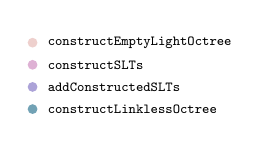
\begin{tikzpicture}
      \node (legend1) at (0.0\textwidth, 0)
            [legend-point, fill={legend1}, label=right:{\tiny $\mathtt{constructEmptyLightOctree}$}] {};
      \node (legend2) at (0.0\textwidth, -8pt)
            [legend-point, fill={legend2}, label=right:{\tiny $\mathtt{constructSLTs}$}] {};
      \node (legend6) at (0.0\textwidth, -16pt)
            [legend-point, fill={legend3}, label=right:{\tiny $\mathtt{addConstructedSLTs}$}] {};
      \node (legend7) at (0.0\textwidth, -24pt)
            [legend-point, fill={legend4}, label=right:{\tiny $\mathtt{constructLinklessOctree}$}] {};
    \end{tikzpicture}
  \end{subfigure}%
  \end{adjustbox}%
  \begin{adjustbox}{minipage=0.4\textwidth, scale=0.6}
    \begin{subfigure}[b]{1.6\textwidth}
      \centering
      \def\svgwidth{\textwidth}
      \input{./img/raw/hs-layered-exec/layered_spaceship-indoor_1260.pdf_tex}
      \caption{Spaceship Indoor - 1260 lichten}
      \vspace{4pt}
      \label{fig:hs-layered-exec:indoor-1260}
    \end{subfigure}
  \end{adjustbox}\hspace{0.125\textwidth} %
%  %
%  \begin{adjustbox}{minipage=\textwidth, scale=0.55}
%    \begin{subfigure}[b]{1.6\textwidth}
%      \centering
%      \def\svgwidth{\textwidth}
%      \input{./img/raw/hs-layered-exec/layered_pipers-alley_1044.pdf_tex}
%      \caption{Piper's Alley - 1044 lichten}
%      \label{fig:hs-layered-exec:alley-1044}
%    \end{subfigure}
%  \end{adjustbox} \\
  %
  \begin{adjustbox}{minipage=0.4\textwidth, scale=0.60}
    \begin{subfigure}[b]{1.6\textwidth}
      \centering
      \def\svgwidth{\textwidth}
      \input{./img/raw/hs-layered-exec/layered_ziggurat-city_1170.pdf_tex}
      \caption{Ziggurat city - 1170 lichten}
      \label{fig:hs-layered-exec:city-1170}
    \end{subfigure}
  \end{adjustbox}
  \caption{\small Construction time of the individual steps of Hashed Shading.}
  \label{fig:hs-layered-exec}
  % ------------------------------------------------------------------------------------------------
  \hspace*{-0.15\textwidth}%
  \begin{subfigure}[t]{0.125\textwidth}
    \tikzstyle{legend-point}=[circle, inner sep=1.25pt]
    \definecolor{GraphBlue}{HTML}{6c8abd}
    \definecolor{GraphGreen}{HTML}{73b584}
    \definecolor{GraphRed}{HTML}{d07175}
    \definecolor{GraphPurple}{HTML}{8172b2}
    \definecolor{GraphYellow}{HTML}{ccb974}
    
    \definecolor{legend1}{HTML}{eed0cd}
    \definecolor{legend2}{HTML}{deb1d4}
    \definecolor{legend3}{HTML}{aca3d8}
    \definecolor{legend4}{HTML}{72a2b5}
    \definecolor{legend5}{HTML}{549874}
    \definecolor{legend6}{HTML}{5d773b}
    \definecolor{legend7}{HTML}{6c4c2e}
    \definecolor{legend8}{HTML}{5c2b3d}
    \definecolor{legend9}{HTML}{311c3b}

    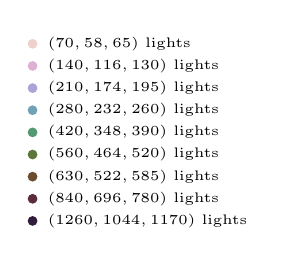
\begin{tikzpicture}
       \node (legend1) at (0.0\textwidth, 0 -4pt)
             [legend-point, fill={legend1}, label=right:{\tiny $(70, 58, 65)$  lights}] {};
       \node (legend2) at (0.0\textwidth, -8pt -4pt)
            [legend-point, fill={legend2}, label=right:{\tiny $(140, 116, 130)$  lights}] {};
      \node (legend3) at (0.0\textwidth, -16pt -4pt)
            [legend-point, fill={legend3}, label=right:{\tiny $(210, 174, 195)$  lights}] {};
      \node (legend4) at (0.0\textwidth, -24pt -4pt)
            [legend-point, fill={legend4}, label=right:{\tiny $(280, 232, 260)$  lights}] {};
      \node (legend5) at (0.0\textwidth, -32pt -4pt)
            [legend-point, fill={legend5}, label=right:{\tiny $(420, 348, 390)$  lights}] {};
      \node (legend6) at (0.0\textwidth, -40pt -4pt)
            [legend-point, fill={legend6}, label=right:{\tiny $(560, 464, 520)$  lights}] {};
      \node (legend7) at (0.0\textwidth, -48pt -4pt)
            [legend-point, fill={legend7}, label=right:{\tiny $(630, 522, 585)$  lights}] {};
      \node (legend8) at (0.0\textwidth, -56pt -4pt)
            [legend-point, fill={legend8}, label=right:{\tiny $(840, 696, 780)$  lights}] {};
      \node (legend9) at (0.0\textwidth, -64pt -4pt)
            [legend-point, fill={legend9}, label=right:{\tiny $(1260, 1044, 1170)$  lights}] {};
    \end{tikzpicture}
  \end{subfigure}%
  \begin{adjustbox}{minipage=0.4\textwidth, scale=0.60}
    \begin{subfigure}[b]{1.6\textwidth}
      \centering
      \def\svgwidth{\textwidth}
      \input{./img/raw/hs-ns-memory/memory_spaceship-indoor.pdf_tex}
      \caption{Spaceship Indoor}
      \vspace{4pt}
      \label{fig:hs-ns-memory:indoor}
    \end{subfigure}
  \end{adjustbox}\hspace{0.125\textwidth} %
  \begin{adjustbox}{minipage=0.4\textwidth, scale=0.60}
    \begin{subfigure}[b]{1.6\textwidth}
      \centering
      \def\svgwidth{\textwidth}
      \input{./img/raw/hs-ns-memory/memory_ziggurat-city.pdf_tex}
      \caption{Ziggurat City}
      \label{fig:hs-ns-memory:city}
    \end{subfigure}
  \end{adjustbox}
  \caption{\small The combined number of pixels of the Linkless Octree.}
  \label{fig:hs-ns-memory}
  % ------------------------------------------------------------------------------------------------
  \hspace*{-0.15\textwidth}%
  \begin{subfigure}[t]{0.125\textwidth}
    \tikzstyle{legend-point}=[circle, inner sep=1.25pt]
    \definecolor{GraphBlue}{HTML}{6c8abd}
    \definecolor{GraphGreen}{HTML}{73b584}
    \definecolor{GraphRed}{HTML}{d07175}
    \definecolor{GraphPurple}{HTML}{8172b2}
    \definecolor{GraphYellow}{HTML}{ccb974}
    
    \definecolor{legend1}{HTML}{eed0cd}
    \definecolor{legend2}{HTML}{deb1d4}
    \definecolor{legend3}{HTML}{aca3d8}
    \definecolor{legend4}{HTML}{72a2b5}
    \definecolor{legend5}{HTML}{549874}
    \definecolor{legend6}{HTML}{5d773b}
    \definecolor{legend7}{HTML}{6c4c2e}
    \definecolor{legend8}{HTML}{5c2b3d}
    \definecolor{legend9}{HTML}{311c3b}

    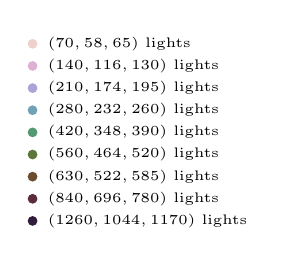
\begin{tikzpicture}
       \node (legend1) at (0.0\textwidth, 0 -4pt)
             [legend-point, fill={legend1}, label=right:{\tiny $(70, 58, 65)$  lights}] {};
       \node (legend2) at (0.0\textwidth, -8pt -4pt)
            [legend-point, fill={legend2}, label=right:{\tiny $(140, 116, 130)$  lights}] {};
      \node (legend3) at (0.0\textwidth, -16pt -4pt)
            [legend-point, fill={legend3}, label=right:{\tiny $(210, 174, 195)$  lights}] {};
      \node (legend4) at (0.0\textwidth, -24pt -4pt)
            [legend-point, fill={legend4}, label=right:{\tiny $(280, 232, 260)$  lights}] {};
      \node (legend5) at (0.0\textwidth, -32pt -4pt)
            [legend-point, fill={legend5}, label=right:{\tiny $(420, 348, 390)$  lights}] {};
      \node (legend6) at (0.0\textwidth, -40pt -4pt)
            [legend-point, fill={legend6}, label=right:{\tiny $(560, 464, 520)$  lights}] {};
      \node (legend7) at (0.0\textwidth, -48pt -4pt)
            [legend-point, fill={legend7}, label=right:{\tiny $(630, 522, 585)$  lights}] {};
      \node (legend8) at (0.0\textwidth, -56pt -4pt)
            [legend-point, fill={legend8}, label=right:{\tiny $(840, 696, 780)$  lights}] {};
      \node (legend9) at (0.0\textwidth, -64pt -4pt)
            [legend-point, fill={legend9}, label=right:{\tiny $(1260, 1044, 1170)$  lights}] {};
    \end{tikzpicture}
  \end{subfigure}%
  \begin{adjustbox}{minipage=0.4\textwidth, scale=0.60}
    \begin{subfigure}[b]{1.6\textwidth}
      \centering
      \def\svgwidth{\textwidth}
      \input{./img/raw/hs-ns-light-indices/light_indices_spaceship-indoor.pdf_tex}
      \caption{Spaceship Indoor}
      \vspace{4pt}
      \label{fig:hs-ns-light-indices:indoor}
    \end{subfigure}
  \end{adjustbox}\hspace{0.125\textwidth} %
  \begin{adjustbox}{minipage=0.4\textwidth, scale=0.60}
    \begin{subfigure}[b]{1.6\textwidth}
      \centering
      \def\svgwidth{\textwidth}
      \input{./img/raw/hs-ns-light-indices/light_indices_ziggurat-city.pdf_tex}
      \caption{Ziggurat City}
      \label{fig:hs-ns-light-indices:city}
    \end{subfigure}
  \end{adjustbox}
  \caption{\small Size of the Light Index List.}
  \label{fig:hs-ns-light-indices}
\end{figure}
